\chapter{Introducción}
Dependiendo del contexto de trabajo, se suelen utilizar diferentes terminologías para referirse a los mismos conceptos. Por ello, antes que nada, se mencionará los términos utilizados para referirnos a diferentes objetivos o problemas basándonos en \cite{2019arXiv190803673W}. \autoref{fig:object-detection}\\

Diremos que estamos en un problema de clasificación de imágenes (global), o \emph{(global) image classification}, cuando se pretenda asignar una única etiqueta a una imagen, de forma que esta categoría represente a toda la imagen o sea la que más se acerque a ella.\\

El siguiente paso, es la detección de objetos, o \emph{object detection}, que será cuando la imagen pueda ser dividida en múltiples cuadros, o \emph{frames}, que serán clasificados con una etiqueta cada uno, obteniendo así múltiples etiquetas para la misma imagen y conociendo la localización correspondiente a cada categoría.\\

Cuando se busca conocer los píxeles concretos pertenecientes a determinada categoría, estaremos ante un problema de segmentación semántica, o \emph{semantic segmentation}, en el que estaremos distinguiendo las regiones de la imagen por el significado que estas pueden conllevar consigo.\\

Finalmente, cuando no sólo se distingue entre qué píxeles pertenecen a determinada categoría sino que también distinguimos cuáles conforman distintos objetos, estaremos ante un problema de instanciación semántica de objetos, o \emph{instance segmentation}.\\

\begin{figure}[htpb]
  \centering
  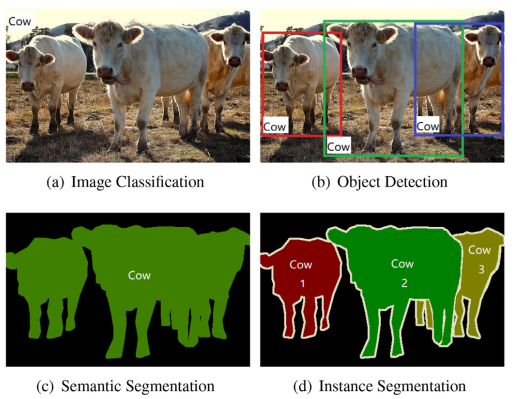
\includegraphics[width=0.65\textwidth]{object_detection}
  \caption{Detección, clasificación y segmentación. \cite{2019arXiv190803673W}}
  \label{fig:object-detection}
\end{figure}

Para indicar las posiciones de los elementos, por lo general se utilizarán \emph{bounding-box} o \emph{bbox} que serán \emph{frames} que contendrán cada uno de los elementos o \emph{pixel level} que colorea cada uno de los píxeles pertenecientes a determinada categoría, ambos con la mayor precisión posible.\\

Hasta este momento, hemos tratado un problema de clasificación global. Se suponía que la imagen tenía un único elemento que se quisiera clasificar e idealmente este estaría centrado con respecto el centro de la imagen. En adelante, querremos clasificar múltiples elementos pertenecientes a múltiples etiquetas distintas y querremos saber cuántos elementos hay, sus posiciones relativas a la imagen y la categoría a la que pertenecen cada una de ellas. En concreto, estaremos ante un problema de segmentación semántica.\\

El objetivo no es utilizar directamente la mejor de las opciones sino explorar otras opciones, ya existentes, que puedan llegar a ser de utilidad en las investigaciones venideras. En particular, nos centraremos en los \emph{non-local block} (\autoref{def:non-local} \autoref{def:non-local-block}) al crear ejemplos de redes neuronales y comprobar el comportamiento ante la eliminación o sustitución de este bloque.\\

Como tampoco debemos olvidarnos de lo que realmente se utiliza, en la siguiente sección hablaremos del estado del arte para la detección de objetos, segmentación semántica e instanciación semántica en conjunto, al ser problemas íntimamente relacionados. Seguidamente mostraremos las estructuras analizadas y algunas de las gráficas obtenidas durante el entrenamiento de estas.

\chapter{Estado del arte}
La gran mayoría de los paradigmas de detección utilizan una red neuronal pre-entrenada como clasificador dentro de sus estructuras. Recibiendo modificaciones en sus últimas capas ya sea sustituyéndolas, pasando por un proceso de \emph{fine-tuning}, o eliminándolas antes de ser añadidas como un elemento invariante durante el entrenamiento del modelo. Estas redes suelen recibir el nombre de \emph{backbone} y algunos modelos permiten la libre elección de estos clasificadores dependiendo del problema concreto que se desee abordar.\newline

En particular, se mencionará dos de las familias más fuertes para la detección en imágenes, la familia RCNN y la famila YOLO.

\section{Dos pasos o basados en RCNN}
El problema de detección se divide en dos etapas: una generación de propuestas y la realización de predicciones sobre estas propuestas. Como paradigmas de detección, destacan la familia \emph{R-CNN} y los que se encuentran basados en esta.\newline

Esta familia surge en noviembre de 2013 con \emph{R-CNN} \cite{2013arXiv1311.2524G} que utiliza Selective Search \cite{Selective Search for object recognition} para generar 2000 \emph{bbox} de propuestas que son redimensionadas para coincidir con las dimensiones de entrada una CNN pre-entrenada. Esta CNN debe volver a entrenarse, extrayéndole la última capa y añadiéndole una \emph{máquina de vectores de soporte (SVM)} con las categorías originales más una nueva clase llamada "fondo" que engloba a todas las propuestas que no pertenecen a ninguna categoría. Finalmente, las propuestas clasificadas son combinadas a través de un modelo de regresión lineal para así obtener una \emph{bbox} con mejor ajuste y precisión.\newline

La principal diferencia que introduce \emph{Fast R-CNN} \cite{2015arXiv150408083G} reside en que, en lugar de pasar por la CNN todas las propuestas de Selective Search, nuestra CNN recibe como entrada la imagen completa reduciendo el coste computacional al analizar una única vez las zonas de solapamiento entre propuestas. Además, las propuestas dejan de ser escaladas para coincidir con una determinada dimensión y se introduce en una capa especial llamada \emph{Region of Interest Pooling Layer (RoI pooling)} que extrae un vector de longitud fija que será la entrada de las siguientes ramas. A continuación, el modelo se divide en dos ramas: un clasificador SoftMax y un modelo de regresión que calcula las \emph{bbox}. \newline

\begin{figure}[htpb]
  \centering
  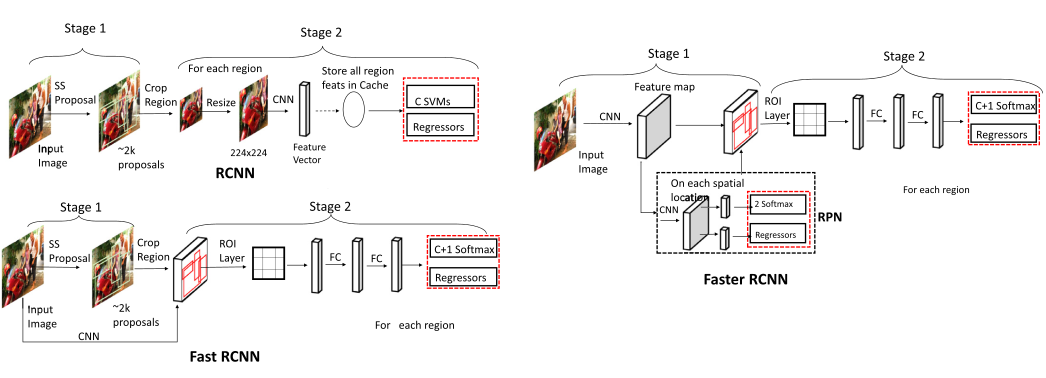
\includegraphics[width=1\textwidth]{rcnn}
  \caption{Comparativa de algunos modelos de la familia R-CNN. \cite{2019arXiv190803673W}}
  \label{fig:r-cnn}
\end{figure}

En \emph{Faster R-CNN} \cite{2015arXiv150601497R} se sustituye Selective Search por una red neuronal de generación propuestas, conocida como \emph{anchor boxes}, que no sólo reduce el tiempo de cómputo de la generación de propuestas sino que aporta un menor número de propuestas con mayor calidad y precisión. Un buen apunte de la red de generación de propuestas es que esta no es pre-entrenada antes de ser añadida al modelo, sino que aprende de forma conjunta con toda la red.\newline

La última mejora de esta familia viene representada por \emph{Mask R-CNN} \cite{2017arXiv170306870H} que sustituye la capa RoI pooling introducida en el modelo Fast R-CNN por una RoI alignment que retiene más información de las características obtenidas por la CNN compartiendo la misma estructura de entrada y salida de datos con la RoI pooling. Mask R-CNN aprovecha esto para realizar predicciones del tipo pixel level con mayor precisión a través de una interpolación bilineal que se ejecuta paralelamente con las capas totalmente conectadas de los modelos anteriores. Así, en el mismo punto que sus predecesores eran divididos en tres ramas independientes, Mask R-CNN se divide en tres ramas: un clasificador SoftMax, un regresor de \emph{bbox} y un otro regresor de pixel level.\newline

%Mencionar Mesh R-CNN
%https://arxiv.org/abs/1906.02739\newline
%Mencionar R-FCN
%https://arxiv.org/pdf/1605.06409.pdf\newline
%Libra R-CNN
%https://arxiv.org/pdf/1904.02701.pdf
\section{Un paso o basados en YOLO}
Estos modelos destacan por no hacer una separación directa de la generación de propuestas y la predicción de estas. Destaca \emph{YOLO} y sus sucesivas mejoras, así como los múltiples algoritmos basados en ellas, pero existen muchos más modelos que pueden ser identificados con esta estructura.\newline

En junio de 2015 aparece \emph{You Only Look Once (YOLO)} \cite{2015arXiv150602640R}, un nuevo algoritmo que pretende realizar al mismo tiempo la generación de propuestas y la clasificación de estas, buscando así una mayor eficiencia computacional. Para ello, tras redimensionar la imagen en 448x448 píxeles, el algoritmo divide la imagen en una cuadrícula cuyas celdas se encargan de realizar un número fijo de propuestas indicando en cada una de ellas la probabilidad que tiene de ser un objeto, la \emph{bbox} en la que se encuentra y la probabilidad de pertenecer a cada una de las clases de objetos de las que disponemos. Finalmente, descarta aquellas propuestas con baja probabilidad de ser un objeto y utiliza un algoritmo de \emph{non-max supression} \cite{2017arXiv170404503B} que unifica y combina las \emph{bbox} con las máximas áreas compartidas.\newline

Buscando una mejora de la predicción pero sin perder el enfoque de la velocidad, surge \emph{YOLO9000} o \emph{YOLOv2} \cite{2016arXiv161208242R} que sigue la misma estructura que su predecesor pero sustituyendo algunos fragmentos por otros con mayor rendimiento. YOLOv2 redimensiona la imagen original a 416x416 píxeles y sustituye las capas totalmente conectadas que utilizaba para la generación de propuestas por un modelo de \emph{anchor boxes} \cite{2015arXiv150601497R} junto con otros cambios menores.\newline

La siguiente versión \emph{YOLOv3} \cite{2018arXiv180402767R} decide  no darle tanta importancia a la velocidad y centrarse en solucionar los problemas de detección presentados por sus antecesores. Mientras que YOLOv2 utiliza una arquitectura con 30 capas, YOLOv3 utiliza 106 capas totalmente convolucionadas e introduce la utilización de \emph{residual blocks}, \emph{skip connections} y \emph{upsampling}. Esta nueva arquitectura, realiza la detección de objetos en tres escalas distintas en diferentes profundidades de la red Darknet-53 y utilizando una estructura piramidal \cite{2016arXiv161203144L} para comunicar la detección entre las diferentes escalas.\newline

%Mencionar YOLOv4
%https://arxiv.org/pdf/2004.10934.pdf\newline

\chapter{Non-local neural networks} \label{def:non-local-block}

En \cite{DBLP:journals/corr/abs-1711-07971} se introduce el concepto de \emph{non-local neural networks} que utiliza una arquitectura ascendente y descendente, \emph{up-down architecture} \cite{2016arXiv160308695P}, para extraer las características de un clasificador a distintos niveles de profundidad y utilizarlas para segmentar semánticamente la imagen \autoref{fig:object-detection}.\newline

\begin{figure}[htpb]
  \centering
  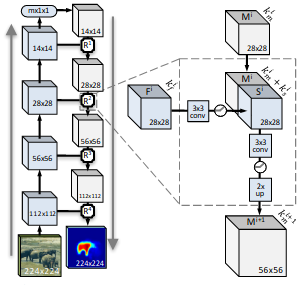
\includegraphics[width=0.6\textwidth]{up-down}
  \caption{Ejemplo de una arquitectura ascendente y descentente con saltos de conexiones\cite{2016arXiv160308695P}.}
  \label{fig:up-down}
\end{figure}


En la parte ascendente de este tipo de arquitecturas nos encontraremos con un clasificador de imágenes, del cual extraeremos información a distintos niveles de profundidad que será unificada y analizada en la parte descendente de la arquitectura para poder predecir los distintos segmentos semánticos. \\

Las \emph{non-local neural networks} se distinguen por la utilización de \emph{non-local block}, o bloques no locales, como extractores de características en los distintos niveles de profundidad. Estos bloques serán de la forma: $$z_i=W f_i(x_i) + x_i,$$  donde $i$ representa el índice de una posición de salida, $x_i$ el $i$-ésimo elemento de la entrada $x$, $f_i$ la $i$-ésima coordenada de una operación no local $f$ (\autoref{def:non-local}) y $W$ un peso que será entrenado por la red. \\

%Podemos distinguir tres tipos de componentes principales: clasificador, bloque no local o \emph{non-local block} y bloque de fusión o \emph{fuse up block}. Lo que más destaca de estas estructuras son los non-local block utilizados para extraer las características puesto que, en lugar obtenerlas utilizando de forma recurrente convoluciones en pequeñas áreas, comprueban las relaciones entre los datos con una única operación que, además, comprueba la afinidad con los datos más distantes.\newline

%A continuación, nos centraremos en los non-local block, definiendo las clase de funciones que los forman y demostrando algunas de sus propiedades que garantizarán su correcto funcionamiento. Seguidamente, mostraremos algunos ejemplos y cómo podemos configurar nuestra propia red según nuestras necesidades.\newline

%\subsection{Non-local block}
%Finalmente, el bloque non-local es de la forma: $$z_i=W_z f(x_i) + x_i,$$ donde multiplicamos la función no local por un peso que será entrenado por la red y le añadimos una conexión residual para evitar perder las características del modelo pre-entrenado en caso de que $W_z$ comience siendo inicializado como $0$.

%FIXME: Añadir más ventajas de la conexión residual.

\chapter{Diseño}

Para el desarrollo de la red neuronal que se ha implementado, se ha utilizado el artículo \emph{Real-time Semantic Segmentation with Fast Attention} \cite{2020arXiv200703815H} publicado el 9 de julio de 2020. En este artículo se busca implementar una red neuronal capaz de realizar segmentación semántica en tiempo real, sin una gran pérdida de precisión y pudiendo ser ejecutada en dispositivos con pocos recursos.\\

Siguiendo sus ideas, se ha utilizado como clasificador un ResNet-18 \cite{DBLP:journals/corr/HeZRS15} para la región ascendente de las \emph{non local neural network} a desarrollar. Como bloque no local \autoref{fig:non-local} se ha utilizado el, que los autores denominan, \emph{fast attention module}, que implementa como operación no local \autoref{def:non-local} una \emph{dot-product similarity} con $v(x_j)=W_{v_j}x_j$ que tendrá la función de extraer y analizar las características del clasificador. \\

\begin{figure}[h]
  \centering
  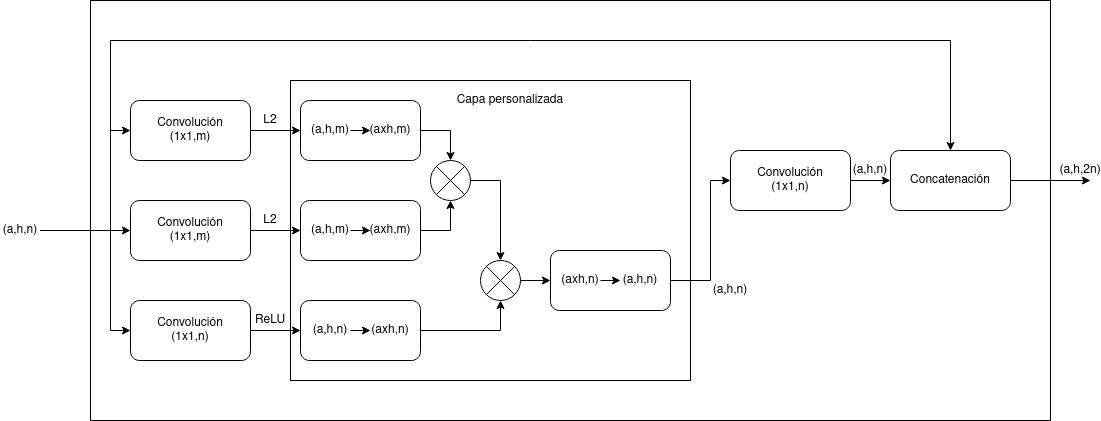
\includegraphics[width=1.05\textwidth]{Nonlocal}
  \caption{Módulo \emph{fast attention}. Diseño implementado del bloque no local \autoref{def:non-local-block} que utiliza la operación no local \autoref{def:non-local} siguiendo \cite{2020arXiv200703815H}.}
  \label{fig:non-local}
\end{figure}

Este módulo permite la fijación del parámetro $m$, correspondiente al número de canales que tendrán las convoluciones que poseen regulación L2 y que serán mantenidas por el resto de operaciones hasta desaparecer esta cantidad por el producto matricial implementado. Por otro lado, el parámetro $n$ corresponderá a los canales de los datos de entrada.\\

A nivel comparativo, como extractor de características, se utilizará también una convolución \autoref{ch:cnn} de núcleo de dimensión $2$. El objetivo será comprobar empíricamente que el número de variables utilizadas no es lo que determinada la efectividad de un modelo, sino el cómo estas son utilizadas. Por ello, se ha decidido utilizar esta capa que es comúnmente utilizada para los problemas que estamos mencionando y que utiliza, únicamente, $4$ variables por cada $3$ utilizadas por el módulo \emph{fast attention} \autoref{fig:non-local} implementado.\\

Para reconstruir las formas a través de las características extraídas nos hemos basado en el modelo U-Net \cite{2015arXiv150504597R}, en particular en la implementación realizada por el tutorial de segmentación de imágenes de Tensorflow \cite{tensorflowTutorial} \autoref{fig:fuse-up}.\\

\begin{figure}[h!]
  \centering
  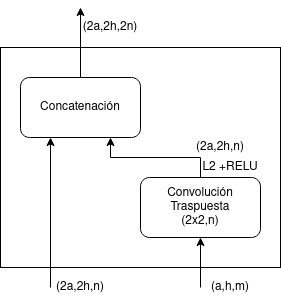
\includegraphics[width=0.4\textwidth]{FuseUP}
  \caption{Diseño implementado del bloque de fusión de capas utilizado para la reconstrucción en la sección descendente de la arquitectura.}
  \label{fig:fuse-up}
\end{figure}

\newpage
Así, como estructura base tendremos:\\

\begin{figure}[h!]
  \centering
  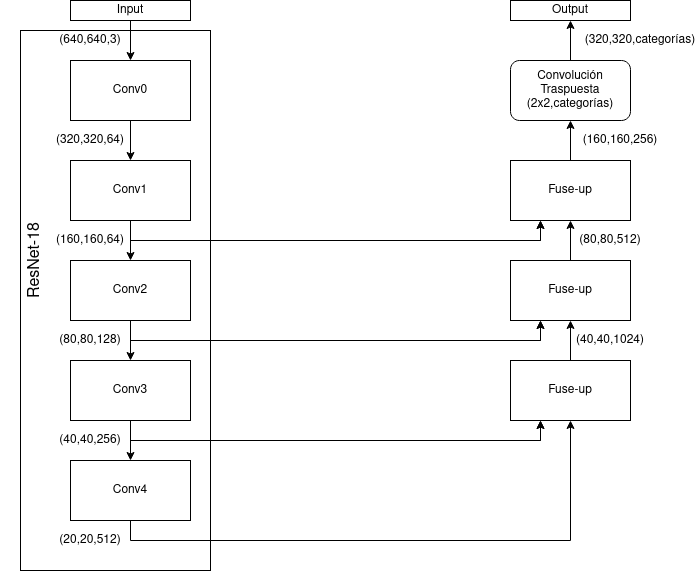
\includegraphics[width=0.9\textwidth]{DiagramaUnet}
  \caption{Diseño base basado en U-net \cite{2015arXiv150504597R} que utiliza como \emph{backbone} una ResNet-18 \cite{DBLP:journals/corr/HeZRS15}.}
  \label{fig:DiagramaUnet}
\end{figure}

\newpage
Que al añadir el bloque no local denominado como módulo \emph{fast attention} queda como:\\

\begin{figure}[h]
  \centering
  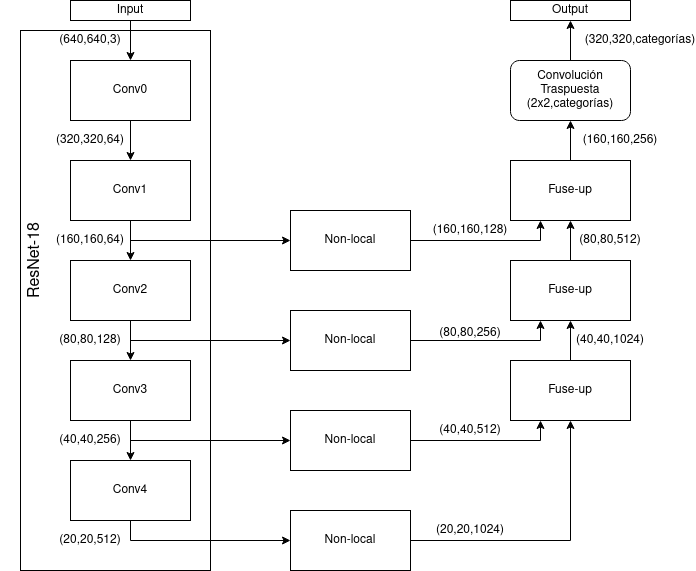
\includegraphics[width=0.9\textwidth]{DiagramaCompleto}
  \caption{Diseño base basado en U-net \cite{2015arXiv150504597R} que utiliza como \emph{backbone} una ResNet-18 \cite{DBLP:journals/corr/HeZRS15}. Utiliza el módulo \autoref{fig:non-local} como extractor de características.}
  \label{fig:DiagramaCompleto}
\end{figure}

\newpage
Sin embargo, en la siguiente sección veremos que al aumentar el número de categorías los resultados decaen. Por ello, se añade una nueva convolución al final de la reconstrucción y se modifica la convolución traspuesta original, con el fin de analizar las características obtenidas en los diferentes niveles de profundidad, quedando la estructura base como:\\

\begin{figure}[h]
  \centering
  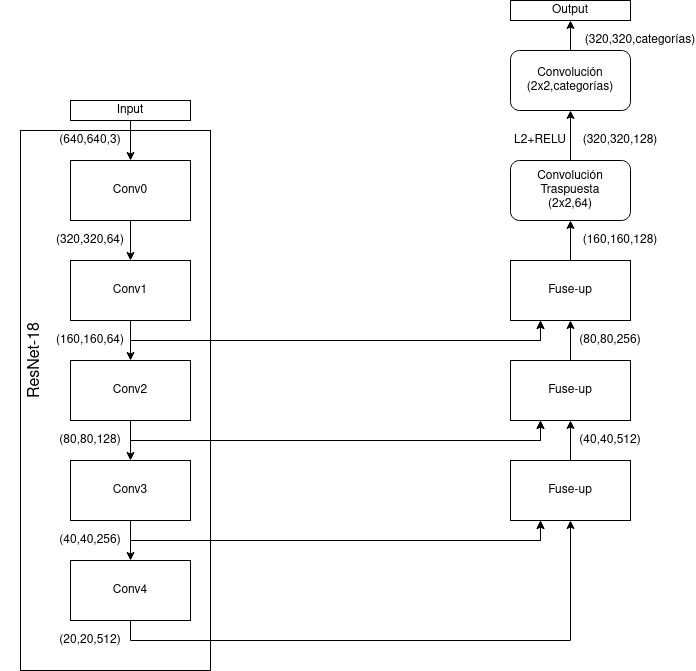
\includegraphics[width=0.9\textwidth]{DiagramaUnetExtra}
  \caption{Diseño base basado en U-net \cite{2015arXiv150504597R} que utiliza como \emph{backbone} una ResNet-18 \cite{DBLP:journals/corr/HeZRS15}. Utiliza una convolución extra al final para analizar la información obtenida y distinguir a través de esta.}
  \label{fig:DiagramaUnetExtra}
\end{figure}

\newpage
Por lo que añadiendo el bloque no local tendremos:\\

\begin{figure}[h]
  \centering
  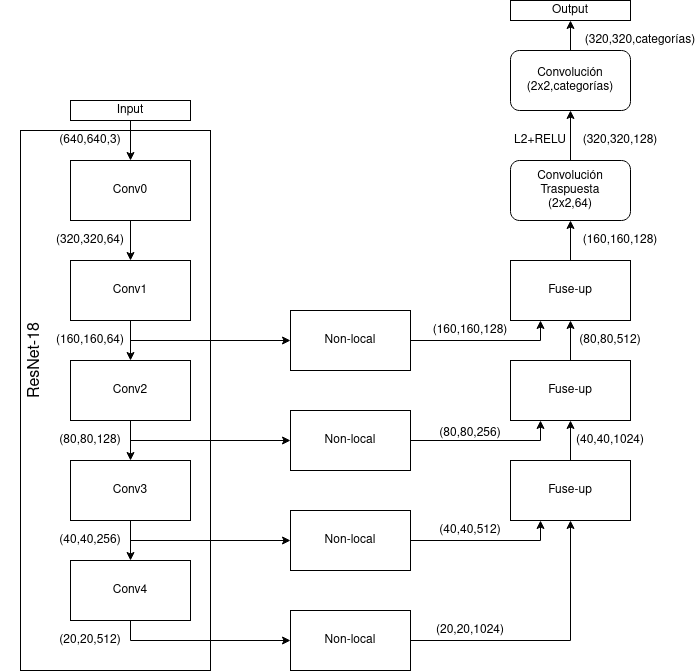
\includegraphics[width=0.9\textwidth]{DiagramaNonlocalExtra}
  \caption{Diseño base basado en U-net \cite{2015arXiv150504597R} que utiliza como \emph{backbone} una ResNet-18 \cite{DBLP:journals/corr/HeZRS15}. Utiliza una convolución extra al final para analizar la información obtenida y distinguir a través de esta. Utiliza el módulo \autoref{fig:non-local} como extractor de características.}
  \label{fig:DiagramaNonlocalExtra}
\end{figure}
\newpage
Y al sustituir el bloque no local como extractor de características por la convolución de núcleo de tamaño $2$ se obtendrá:\\

\begin{figure}[h]
  \centering
  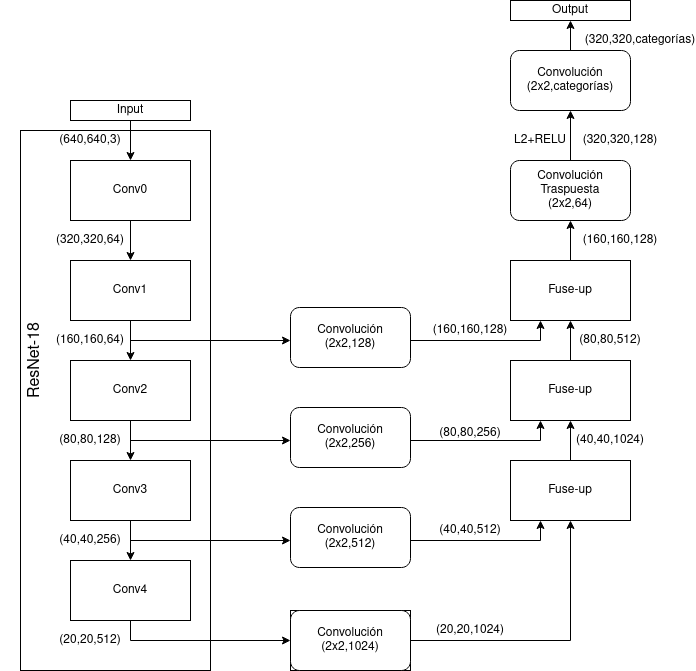
\includegraphics[width=0.9\textwidth]{DiagramaConvExtra}
  \caption{Diseño base basado en U-net \cite{2015arXiv150504597R} que utiliza como \emph{backbone} una ResNet-18 \cite{DBLP:journals/corr/HeZRS15}. Utiliza una convolución extra al final para analizar la información obtenida y distinguir a través de esta. Utiliza convoluciones de núcleo de tamaño $2$ como extractor de características.}
  \label{fig:DiagramaConvExtra}
\end{figure}

\newpage
Al añadir otro bloque de \emph{fuse up} surgió la posibilidad de que, añadiendo otro bloque no local, se consiguiera mejorar los resultados. Como se verá en la siguiente sección, no fue así.\\

\begin{figure}[h]
  \centering
  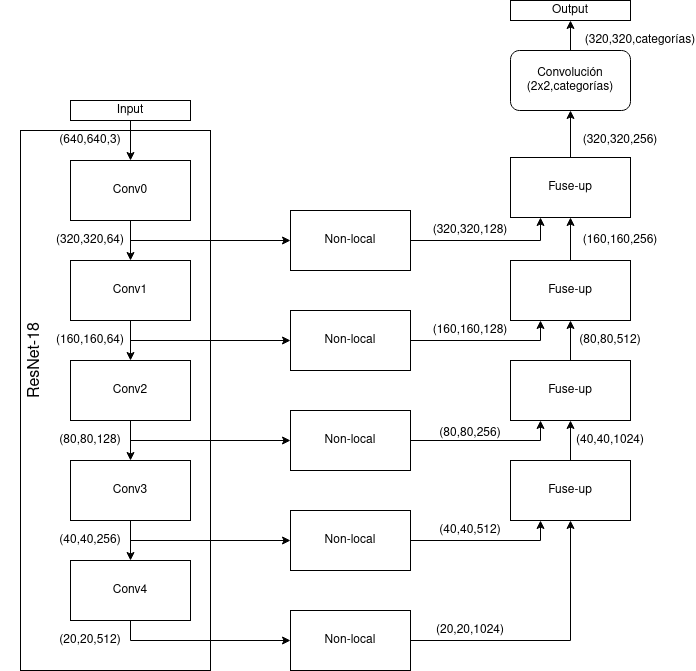
\includegraphics[width=0.9\textwidth]{DiagramaNonlocal+Extra}
  \caption{Diseño base basado en U-net \cite{2015arXiv150504597R} que utiliza como \emph{backbone} una ResNet-18 \cite{DBLP:journals/corr/HeZRS15}. Utiliza una convolución extra al final para analizar la información obtenida y distinguir a través de esta. Utiliza el módulo \autoref{fig:non-local} como extractor de características y posee un módulo extra.}
  \label{fig:DiagramaNonlocal+Extra}
\end{figure}

\newpage
Ante la posibilidad anterior, y su resultado, se diseñó otro planteamiento que veía reducido su número de bloques no locales, sin llegar a eliminarlos todos, para poder observar cómo esta reducción afectaba a la segmentación y si era necesario, o no, la utilización de todos los bloques.\\

\begin{figure}[h]
  \centering
  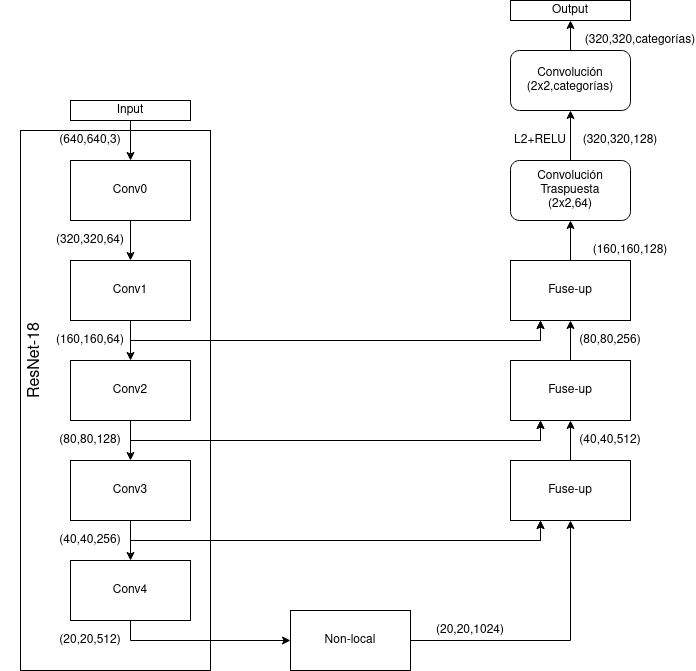
\includegraphics[width=0.9\textwidth]{DiagramaSemiNonlocalExtra}
  \caption{Diseño base basado en U-net \cite{2015arXiv150504597R} que utiliza como \emph{backbone} una ResNet-18 \cite{DBLP:journals/corr/HeZRS15}. Utiliza una convolución extra al final para analizar la información obtenida y distinguir a través de esta. Utiliza el módulo \autoref{fig:non-local} como extractor de características en la máxima profundidad.}
  \label{fig:DiagramaSemiNonlocalExtra}
\end{figure}

\newpage
Y comprobaremos también esta posibilidad utilizando la convolución de núcleo de tamaño $2$:
\begin{figure}[h]
  \centering
  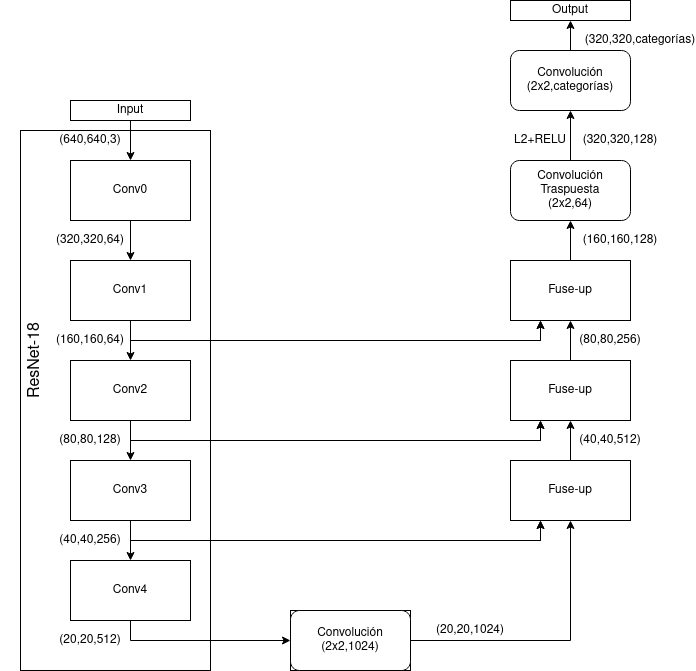
\includegraphics[width=0.9\textwidth]{DiagramaSemiConvExtra}
  \caption{Diseño base basado en U-net \cite{2015arXiv150504597R} que utiliza como \emph{backbone} una ResNet-18 \cite{DBLP:journals/corr/HeZRS15}. Utiliza una convolución extra al final para analizar la información obtenida y distinguir a través de esta. Utiliza convoluciones de núcleo de tamaño $2$ como extractor de características en la máxima profundidad.}
  \label{fig:DiagramaSemiConvExtra}
\end{figure}

\chapter{Experimentos}

\section{Parámetros y configuración de entrenamiento}
Como función de pérdida se ha utilizado la \emph{Sparse Categorial Crossentropy} ofrecida por Keras \cite{chollet2015keras}. Esta función aplica una función \emph{SoftMax} a la salida de la red antes de calcular su entropía cruzada. Se diferencia de la \emph{Categorical Crossentropy} por el formato de entrada de las etiquetas verdaderas, al requerir una matriz bidimensional en lugar de una tridimensional con el fin de reducir el cómputo. \\

El optimizador empleado será \emph{Adam}, con los parámetros por defecto, e iremos reduciendo el ratio de aprendizaje un factor de $0.1$ cada $3$ épocas sin reducir la pérdida en el conjunto de validación hasta un valor mínimo de $10^{-10}$. Además, si ocurren $10$ épocas y no mejora el valor de pérdida en el conjunto de validación, el entrenamiento se detendrá al interpretarse que ha llegado a su límite y no será capaz de aprender mucho más. Cada vez que obtengamos un mejor valor de pérdida en el conjunto de validación, se guardarán los pesos que posea la red neuronal en dicho momento.\\

Como métrica, se utilizará \emph{Mean IoU}, o media de la intersección sobre la unión, en lugar de la clásica \emph{accuracy}, puesto que será la que realmente prediga cómo de bien se comporta la red. Esto es debido a que podríamos predecir que no existe ningún objeto en la imagen y obtener una precisión alta cuando realmente existen pequeños objetos que no han sido predichos. En \cite{accvsiou} se puede ver una explicación más detallada de este fenómeno y el por qué del uso de la intersección sobre la unión. \\

Como conjunto de datos de entrenamiento, se ha utilizado COCO 2017 \cite{2014arXiv1405.0312L} \cite{COCO} que posee un total de 91 categorías correspondientes a objetos del día a día. Estas categorías pueden ser agrupadas en hiper categorías, de forma que se realizarán entrenamientos con todo el conjunto de datos y también con aquellos pertenecientes a la hiper categorías de transportes. El objetivo es comparar el comportamiento en diferentes cantidades de categorías a aprender.\\

Para incrementar la variedad de imágenes sin aumentar la cantidad de estas, buscando obtener una mayor generalidad de la red sin aumentar el cómputo, se implementarán una serie de transformaciones de los datos. Esto será la aplicación de un conjunto de transformaciones a las imágenes originales y a sus máscaras de etiquetas cada vez que estas sean consultadas para el entrenamiento. \\

\newpage
En particular, se aplicarán, en orden, entre una o dos transformaciones de las siguientes opciones \cite{imgaug}: \\
\begin{itemize}
\item Reflejo horizontal. En caso  de salir esta opción, tendrá una probabilidad de $0.5$ de ser aplicado.
\item Escalado. La imagen será escalada de forma aleatoria, como mínimo será la mitad de su escala original y como máximo se verá incrementada un $50\%$.
\item Traslación. La imagen será trasladada entre el $-20\%$ y el $+20\%$ de su tamaño, representando un valor negativo la traslación hacia la izquierda y un valor positivo la traslación hacia la derecha.
\end{itemize}

Se pueden llegar a aplicar muchas más operaciones para la transformación de datos, pero se ha decidido utilizar estas que son fácilmente interpretables y que, por el contexto actual de imágenes, no insertan información conflictiva tras la transformación. Un ejemplo de transformación a evitar sería el reflejo vertical, que podría dar como resultado tener el cielo abajo y un bosque arriba de este. No es esperable recibir imágenes de este tipo, y por ello entrenar la red para tenerlas en cuenta podría emitir peores resultados.\\

Todas las gráficas e imágenes comparativas que utilizaremos en futuras secciones se podrán encontrar en diversos cuadernillos de \emph{jupyter notebook}, que podrán ser encontrados dentro de las subcarpetas localizadas en \emph{modelos-entrenados} junto con los archivos de pesos y del historial del entrenamiento guardados. Todo esto puede ser encontrado en el repositorio de GitHub del proyecto \cite{GitHub}.\\

%\begin{figure}[htpb]
%  \centering
%  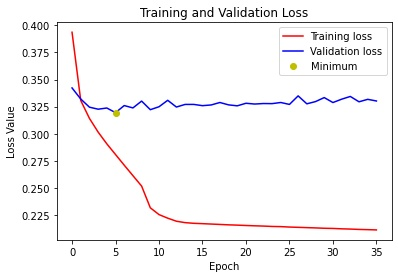
\includegraphics[width=0.48\textwidth]{../../modelos-entrenados/unet/ejecucion1/lossUnet}
%  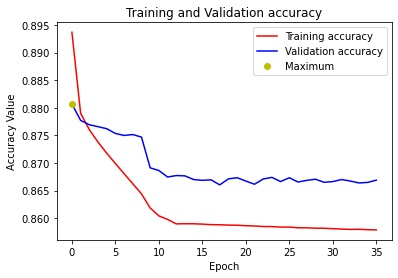
\includegraphics[width=0.48\textwidth]{../../modelos-entrenados/unet/ejecucion1/accUnet}
%  \caption{Entrenamiento del modelo mostrado en \autoref{fig:DiagramaUnet} sin transformación de datos y sin detención temprana. Subcategoría de Transportes.}
%  \label{fig:ejec1}
%\end{figure}

%\begin{figure}[htpb]
%  \centering
%  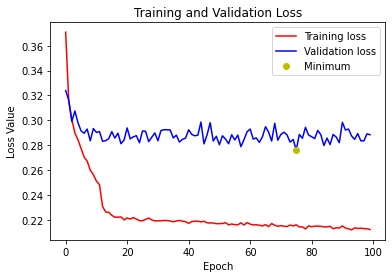
\includegraphics[width=0.48\textwidth]{../../modelos-entrenados/unet/ejecucion2/lossUnet2}
%  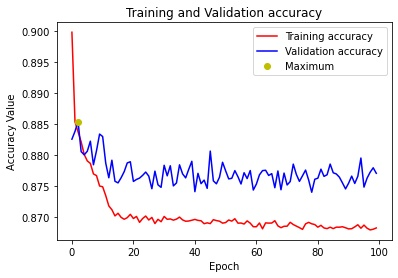
\includegraphics[width=0.48\textwidth]{../../modelos-entrenados/unet/ejecucion2/accUnet2}
%  \caption{Entrenamiento del modelo mostrado en \autoref{fig:DiagramaUnet} con transformación de datos tanto en los datos de entrenamiento como en los de validación. Subcategoría de Transportes.}
%  \label{fig:ejec2}
%\end{figure}

%\begin{figure}[htpb]
%  \centering
%  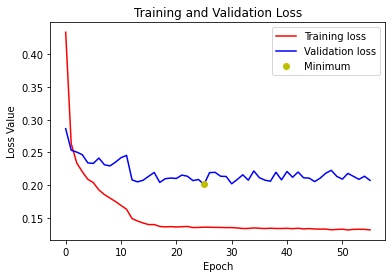
\includegraphics[width=0.48\textwidth]{../../modelos-entrenados/unet-nonlocal/ejecucion3/loss}
%  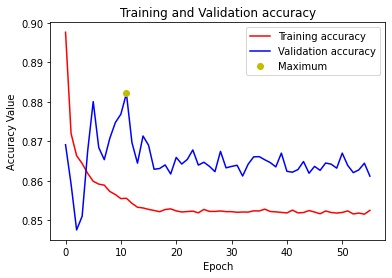
\includegraphics[width=0.48\textwidth]{../../modelos-entrenados/unet-nonlocal/ejecucion3/acc}
%  \caption{Entrenamiento del modelo mostrado en \autoref{fig:DiagramaCompleto} con transformación de datos tanto en los datos de entrenamiento como en los de validación. $64$ canales en el bloque de atención. Subcategoría de Transportes.}
%  \label{fig:ejec3}
%\end{figure}

\section{Análisis}

Debido a la cantidad de gráficas, se irá seleccionando diferentes combinaciones a comparar, con el fin de resaltar de forma específica qué se quería analizar en cada momento. De esta forma, nos iremos centrando en las diferencias presentes en cada modelo entrenado y se podrá ver si estas diferencias afectan de forma significativa al resultado y, en caso de afectar, cómo lo hace.\\
\begin{figure}[h]
  \centering
  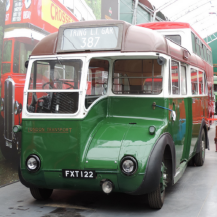
\includegraphics[width=0.35\textwidth]{../../modelos-entrenados/unet-conv/ejecucion12/img1}
  \vrule
  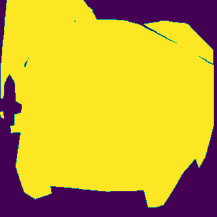
\includegraphics[width=0.35\textwidth]{../../modelos-entrenados/unet-conv/ejecucion12/img-ann1}
  \vrule
  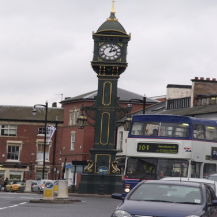
\includegraphics[width=0.35\textwidth]{../../modelos-entrenados/unet-conv/ejecucion12/val2}
  \vrule
  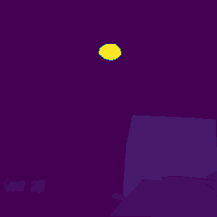
\includegraphics[width=0.35\textwidth]{../../modelos-entrenados/unet-conv/ejecucion12/val-ann2}
  \caption{Imágenes de muestra utilizada en las futuras comparativas. A la izquierda la imagen redimensionada y a la derecha las máscaras verdaderas correspondientes. Arriba conjunto de entrenamiento y abajo conjunto de validación. Cada color distinto representa una capa en las máscaras veraderas.}
  \label{fig:imagenes-muestra}
\end{figure}

Además de las gráficas, también se utilizarán las imágenes mostradas en \autoref{fig:imagenes-muestra} como comparativa de resultados en diferentes ocasiones. Debemos mencionar también que las máscaras verdaderas están almacenadas como imágenes en escala de grises donde cada valor representa a una categoría en concreto y, teniendo en cuenta el método de visualización elegido, siempre se mostrará el mayor valor en color amarillo mientras que los colores más pequeños se irán tornando más azulados. En concreto el valor $0$ corresponde a la ausencia de objetos y se muestra como un color azul oscuro en las imágenes de máscaras verdaderas.\\

\newpage
La representación por colores mencionada en las máscaras verdaderas, debemos de diferenciarlas de la representación utilizada para la comparativa entre predicción y verdadero valor para una máscara concreta, donde se analiza una única categoría en lugar de mostrar los píxeles de todas ellas. En este caso, el color azul intermedio corresponderá a las predicciones y el color amarillo a los falsos negativos.\\

\newpage
\subsection{Diferentes cantidades de bloques no locales.}
Lo primero a comparar será los resultados obtenidos dependiendo de la cantidad de módulos no locales empleados en la red. En particular, se observarán las gráficas \autoref{fig:ejec10}, \autoref{fig:ejec9} y \autoref{fig:ejec11} que únicamente se diferencian en dicha cantidad.\\

\begin{figure}[h!]
  \centering
  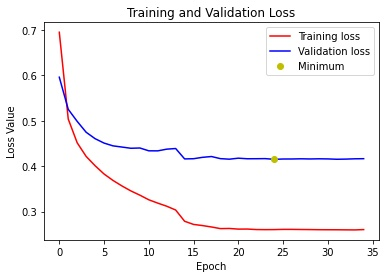
\includegraphics[width=0.48\textwidth]{../../modelos-entrenados/unet-nonlocal-conv/ejecucion10/loss}
  %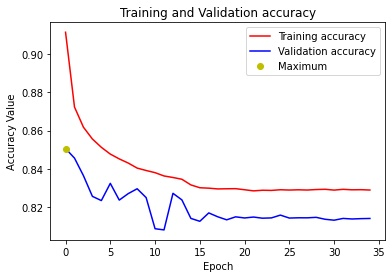
\includegraphics[width=0.48\textwidth]{../../modelos-entrenados/unet-nonlocal-conv/ejecucion10/acc}
  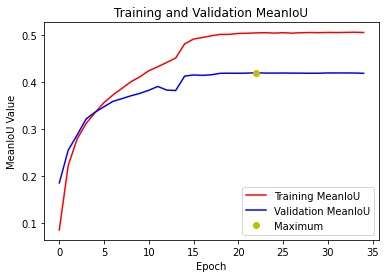
\includegraphics[width=0.48\textwidth]{../../modelos-entrenados/unet-nonlocal-conv/ejecucion10/iou}
  \caption{Entrenamiento del modelo mostrado en \autoref{fig:DiagramaNonlocalExtra} con transformación de datos en los datos de entrenamiento. $64$ canales en el bloque de atención. Conjunto de datos completo.}
  \label{fig:ejec10}
\end{figure}

\end{figure}
\begin{figure}[h!]
  \centering
  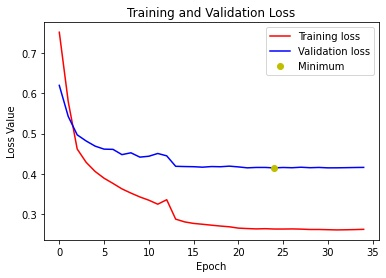
\includegraphics[width=0.48\textwidth]{../../modelos-entrenados/unet-nonlocalextra-conv/ejecucion9/loss}
  %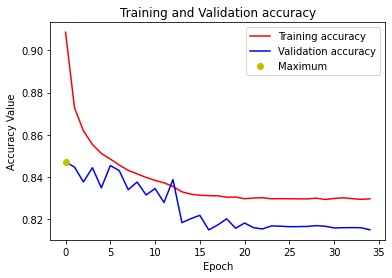
\includegraphics[width=0.48\textwidth]{../../modelos-entrenados/unet-nonlocalextra-conv/ejecucion9/acc}
  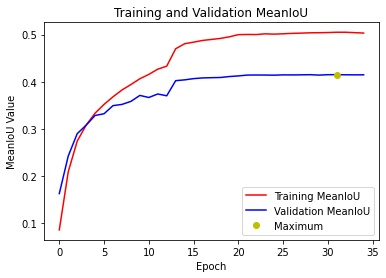
\includegraphics[width=0.48\textwidth]{../../modelos-entrenados/unet-nonlocalextra-conv/ejecucion9/iou}
  \caption{Entrenamiento del modelo mostrado en \autoref{fig:DiagramaNonlocal+Extra} con transformación de datos en los datos de entrenamiento. $64$ canales en el bloque de atención. Conjunto de datos completo.}
  \label{fig:ejec9}
\end{figure}

\begin{figure}[h!]
  \centering
  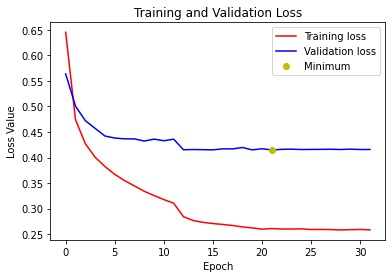
\includegraphics[width=0.48\textwidth]{../../modelos-entrenados/unet-semnonlocal-conv/ejecucion11/loss}
  %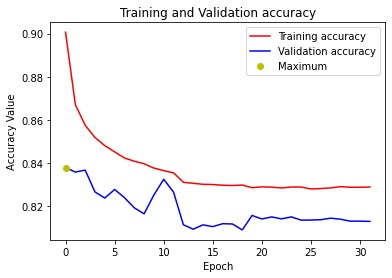
\includegraphics[width=0.48\textwidth]{../../modelos-entrenados/unet-semnonlocal-conv/ejecucion11/acc}
  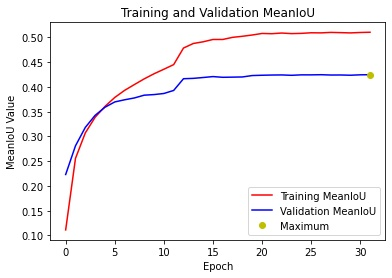
\includegraphics[width=0.48\textwidth]{../../modelos-entrenados/unet-semnonlocal-conv/ejecucion11/iou}
  \caption{Entrenamiento del modelo mostrado en \autoref{fig:DiagramaSemiNonlocalExtra} con transformación de datos en los datos de entrenamiento. $64$ canales en el bloque de atención. Conjunto de datos completo.}
  \label{fig:ejec11}
\end{figure}
Las gráficas correspondientes tienen una estructura similar, siendo que en las 3 se alcanza el mínimo valor de pérdida en el conjunto de validación entre las épocas 20 y 25. Además, en los tres modelos existe un aumento  sustancial del valor medio de la intersección sobre la unión en el conjunto de validación entre las épocas 10 y 15, siendo que este coincide con la primera reducción del ratio de aprendizaje por llevar 3 épocas sin que viera reducido la pérdida en la validación.\\

\newpage
A pesar de seguir realizándose reducciones del ratio de aprendizaje ante la falta de mejoría, no vuelven a producirse mejoras sustanciales durante el aprendizaje en ninguna de ellas.\\

Teniendo en cuenta esto, se comprueba empíricamente que no por añadir más cantidad de bloques no locales se podrán extraer más características de la imagen. Pero, además, debemos de tener en cuenta la gráfica \autoref{fig:ejec12}, correspondiente a la misma arquitectura pero sin bloques no locales, por lo que estos bloques sí establecen una mejoría ante la inexistencia de ningún otro.\\

\begin{figure}[h!]
  \centering
  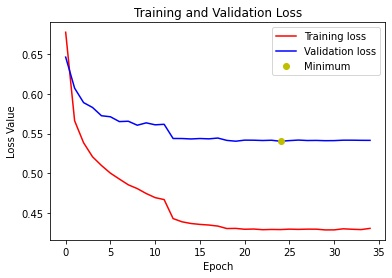
\includegraphics[width=0.48\textwidth]{../../modelos-entrenados/unet-conv/ejecucion12/loss}
  %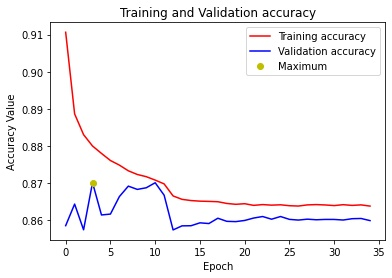
\includegraphics[width=0.48\textwidth]{../../modelos-entrenados/unet-conv/ejecucion12/acc}
  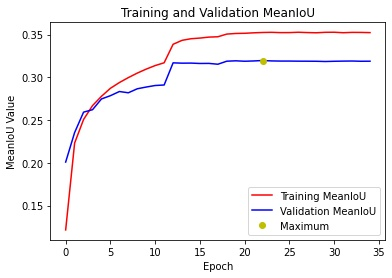
\includegraphics[width=0.48\textwidth]{../../modelos-entrenados/unet-conv/ejecucion12/iou}
  \caption{Entrenamiento del modelo mostrado en \autoref{fig:DiagramaUnetExtra} con transformación de datos en los datos de entrenamiento. $64$ canales en el bloque de atención. Conjunto de datos completo.}
  \label{fig:ejec12}
\end{figure}

\newpage
De forma visual, se puede comprobar tanto en \autoref{fig:comparativa1-train}, que pertenece al conjunto de entrenamiento y muestra la salida de las capas ``nada'' y la capa ``autobús'', como en \autoref{fig:comparativa1-val}, que muestra el resultado de las capas ``nada'', ``coche'', ``autobús'' y ``reloj'' en una imagen perteneciente al conjunto de validación.\\

\begin{figure}[h!tpb]
  \centering
  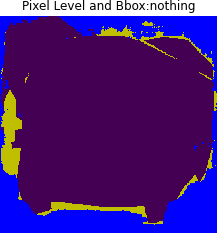
\includegraphics[width=0.2\textwidth]{../../modelos-entrenados/unet-nonlocal-conv/ejecucion10/predtrainmid0}
  \vrule
  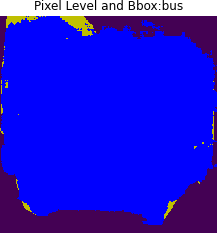
\includegraphics[width=0.2\textwidth]{../../modelos-entrenados/unet-nonlocal-conv/ejecucion10/predtrainmid6}
  \vrule
  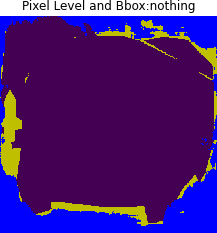
\includegraphics[width=0.2\textwidth]{../../modelos-entrenados/unet-nonlocalextra-conv/ejecucion9/predtrainmid0}
  \vrule
  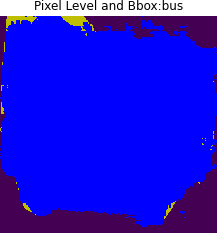
\includegraphics[width=0.2\textwidth]{../../modelos-entrenados/unet-nonlocalextra-conv/ejecucion9/predtrainmid6}
  \vrule
  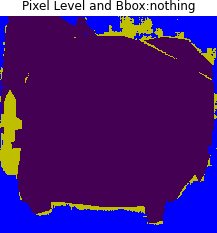
\includegraphics[width=0.2\textwidth]{../../modelos-entrenados/unet-semnonlocal-conv/ejecucion11/predtrainmid0}
  \vrule
  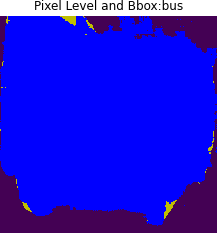
\includegraphics[width=0.2\textwidth]{../../modelos-entrenados/unet-semnonlocal-conv/ejecucion11/predtrainmid6}
  \vrule
  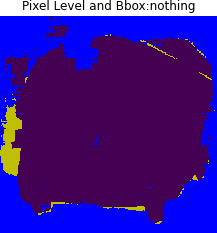
\includegraphics[width=0.2\textwidth]{../../modelos-entrenados/unet-conv/ejecucion12/predtrainmid0}
  \vrule
  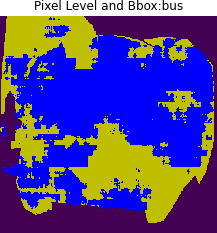
\includegraphics[width=0.2\textwidth]{../../modelos-entrenados/unet-conv/ejecucion12/predtrainmid6}
  \caption{Comparativa con una imagen del conjunto de entrenamiento. Mostradas las capas correspondientes a etiquetas no vacías para la imagen actual. En este caso esta partido en pares, siendo cada par capas el resultado de la predicción de un entrenamiento. De izquierda a derecha y de arriba a abajo, corresponde con las gráficas: \autoref{fig:ejec10}, \autoref{fig:ejec9}, \autoref{fig:ejec11} y \autoref{fig:ejec12}.}
  \label{fig:comparativa1-train}
\end{figure}

\begin{figure}[h!tpb]
  \centering
  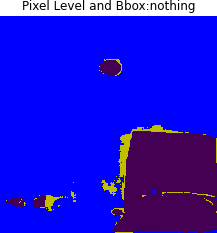
\includegraphics[width=0.2\textwidth]{../../modelos-entrenados/unet-nonlocal-conv/ejecucion10/predvalmid0}
  \vrule
  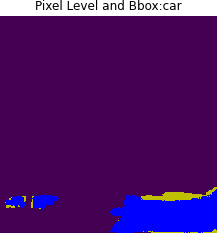
\includegraphics[width=0.2\textwidth]{../../modelos-entrenados/unet-nonlocal-conv/ejecucion10/predvalmid3}
  \vrule
  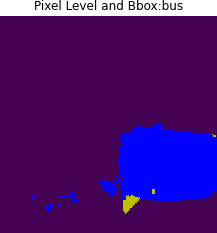
\includegraphics[width=0.2\textwidth]{../../modelos-entrenados/unet-nonlocal-conv/ejecucion10/predvalmid6}
  \vrule
  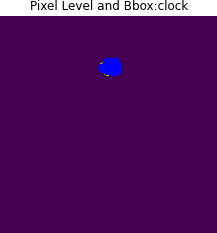
\includegraphics[width=0.2\textwidth]{../../modelos-entrenados/unet-nonlocal-conv/ejecucion10/predvalmid85}
  \vrule
  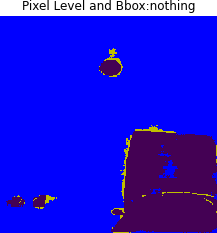
\includegraphics[width=0.2\textwidth]{../../modelos-entrenados/unet-nonlocalextra-conv/ejecucion9/predvalmid0}
  \vrule
  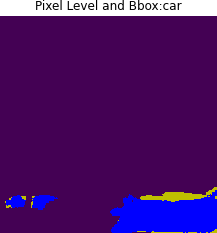
\includegraphics[width=0.2\textwidth]{../../modelos-entrenados/unet-nonlocalextra-conv/ejecucion9/predvalmid3}
  \vrule
  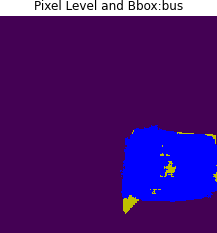
\includegraphics[width=0.2\textwidth]{../../modelos-entrenados/unet-nonlocalextra-conv/ejecucion9/predvalmid6}
  \vrule
  \includegraphics[width=0.2\textwidth]{../../modelos-entrenados/unet-nonlocalextra-conv/ejecucion9/predvalmid85}
  \vrule
  \includegraphics[width=0.2\textwidth]{../../modelos-entrenados/unet-semnonlocal-conv/ejecucion11/predvalmid0}
  \vrule
  \includegraphics[width=0.2\textwidth]{../../modelos-entrenados/unet-semnonlocal-conv/ejecucion11/predvalmid3}
  \vrule
  \includegraphics[width=0.2\textwidth]{../../modelos-entrenados/unet-semnonlocal-conv/ejecucion11/predvalmid6}
  \vrule
  \includegraphics[width=0.2\textwidth]{../../modelos-entrenados/unet-semnonlocal-conv/ejecucion11/predvalmid85}
  \vrule
  \includegraphics[width=0.2\textwidth]{../../modelos-entrenados/unet-conv/ejecucion12/predvalmid0}
  \vrule
  \includegraphics[width=0.2\textwidth]{../../modelos-entrenados/unet-conv/ejecucion12/predvalmid3}
  \vrule
  \includegraphics[width=0.2\textwidth]{../../modelos-entrenados/unet-conv/ejecucion12/predvalmid6}
  \vrule
  \includegraphics[width=0.2\textwidth]{../../modelos-entrenados/unet-conv/ejecucion12/predvalmid85}
  \caption{Comparativa con una imagen del conjunto de validación. Mostradas las capas correspondientes a etiquetas no vacías para la imagen actual. En este caso, cada fila corresponde a las predicciones para de la imagen en un entrenamiento concreto. De arriba a abajo, corresponde con las gráficas: \autoref{fig:ejec10}, \autoref{fig:ejec9}, \autoref{fig:ejec11} y \autoref{fig:ejec12}.}
  \label{fig:comparativa1-val}
\end{figure}
\newpage
\subsection{Bloque no locales y convoluciones}
De forma similar a como pasaba teniendo diferentes cantidades de bloques no locales, tener distintas cantidades de convoluciones como extractores de características no aporta una diferencia significativa en los resultados de entrenamiento, como podemos ver en \autoref{fig:ejec14} y \autoref{fig:ejec13}. \\

\begin{figure}[h!]
  \centering
  \includegraphics[width=0.48\textwidth]{../../modelos-entrenados/unet-conv-conv/ejecucion14/loss}
  %\includegraphics[width=0.48\textwidth]{../../modelos-entrenados/unet-conv-conv/ejecucion14/acc}
  \includegraphics[width=0.48\textwidth]{../../modelos-entrenados/unet-conv-conv/ejecucion14/iou}
  \caption{Entrenamiento del modelo mostrado en \autoref{fig:DiagramaConvExtra} con transformación de datos en los datos de entrenamiento. $64$ canales en convoluciones extractoras. Conjunto de datos completo.}
  \label{fig:ejec14}
\end{figure}

\begin{figure}[h!]
  \centering
  \includegraphics[width=0.48\textwidth]{../../modelos-entrenados/unet-semconv-conv/ejecucion13/loss}
  %\includegraphics[width=0.48\textwidth]{../../modelos-entrenados/unet-semconv-conv/ejecucion13/acc}
  \includegraphics[width=0.48\textwidth]{../../modelos-entrenados/unet-semconv-conv/ejecucion13/iou}
  \caption{Entrenamiento del modelo mostrado en \autoref{fig:DiagramaSemiConvExtra} con transformación de datos en los datos de entrenamiento. $64$ canales en convoluciones extractoras. Conjunto de datos completo.}
  \label{fig:ejec13}
\end{figure}

A pesar de ello, el cambio sí afecta a la velocidad de convergencia del entrenamiento siendo que se produce una buena mejora entre las épocas 25 y 30 en \autoref{fig:ejec13} mientras que en \autoref{fig:ejec14} se produce entre la época 30 y 40.\\
\newpage
De forma visual, se puede comprobar tanto en \autoref{fig:comparativa2-train}, que pertenece al conjunto de entrenamiento y muestra la salida de las capas ``nada'' y la capa ``autobús'', como en \autoref{fig:comparativa2-val}, que muestra el resultado de las capas ``nada'', ``coche'', ``autobús'' y ``reloj'' en una imagen perteneciente al conjunto de validación.\\

\begin{figure}[h!]
  \centering
  \includegraphics[width=0.2\textwidth]{../../modelos-entrenados/unet-conv/ejecucion12/predtrainmid0}
  \vrule
  \includegraphics[width=0.2\textwidth]{../../modelos-entrenados/unet-conv/ejecucion12/predtrainmid6}
  \vrule
  \includegraphics[width=0.2\textwidth]{../../modelos-entrenados/unet-conv-conv/ejecucion14/predtrainmid0}
  \vrule
  \includegraphics[width=0.2\textwidth]{../../modelos-entrenados/unet-conv-conv/ejecucion14/predtrainmid6}
  \vrule
  \includegraphics[width=0.2\textwidth]{../../modelos-entrenados/unet-semconv-conv/ejecucion13/predtrainmid0}
  \vrule
  \includegraphics[width=0.2\textwidth]{../../modelos-entrenados/unet-semconv-conv/ejecucion13/predtrainmid6}
  \caption{Comparativa con una imagen del conjunto de entrenamiento. Mostradas las capas correspondientes a etiquetas no vacías para la imagen actual. En este caso esta partido en pares, siendo cada capa el resultado de la predicción de un entrenamiento. De izquierda a derecha y de arriba a abajo, corresponde con las gráficas: \autoref{fig:ejec12}, \autoref{fig:ejec14} y \autoref{fig:ejec13}.}
  \label{fig:comparativa2-train}
\end{figure}

\begin{figure}[h!]
  \centering
  \includegraphics[width=0.2\textwidth]{../../modelos-entrenados/unet-conv/ejecucion12/predvalmid0}
  \vrule
  \includegraphics[width=0.2\textwidth]{../../modelos-entrenados/unet-conv/ejecucion12/predvalmid3}
  \vrule
  \includegraphics[width=0.2\textwidth]{../../modelos-entrenados/unet-conv/ejecucion12/predvalmid6}
  \vrule
  \includegraphics[width=0.2\textwidth]{../../modelos-entrenados/unet-conv/ejecucion12/predvalmid85}
  \vrule
  \includegraphics[width=0.2\textwidth]{../../modelos-entrenados/unet-conv-conv/ejecucion14/predvalmid0}
  \vrule
  \includegraphics[width=0.2\textwidth]{../../modelos-entrenados/unet-conv-conv/ejecucion14/predvalmid3}
  \vrule
  \includegraphics[width=0.2\textwidth]{../../modelos-entrenados/unet-conv-conv/ejecucion14/predvalmid6}
  \vrule
  \includegraphics[width=0.2\textwidth]{../../modelos-entrenados/unet-conv-conv/ejecucion14/predvalmid85}
  \vrule
  \includegraphics[width=0.2\textwidth]{../../modelos-entrenados/unet-semconv-conv/ejecucion13/predvalmid0}
  \vrule
  \includegraphics[width=0.2\textwidth]{../../modelos-entrenados/unet-semconv-conv/ejecucion13/predvalmid3}
  \vrule
  \includegraphics[width=0.2\textwidth]{../../modelos-entrenados/unet-semconv-conv/ejecucion13/predvalmid6}
  \vrule
  \includegraphics[width=0.2\textwidth]{../../modelos-entrenados/unet-semconv-conv/ejecucion13/predvalmid85}
  \caption{Comparativa con una imagen del conjunto de validación. Mostradas las capas correspondientes a etiquetas no vacías para la imagen actual. En este caso, cada fila corresponde a las predicciones para de la imagen en un entrenamiento concreto. De arriba a abajo, corresponde con las gráficas: \autoref{fig:ejec12}, \autoref{fig:ejec14} y \autoref{fig:ejec13}.}
  \label{fig:comparativa2-val}
\end{figure}

\newpage
Aunque no existe una mejora tan significativa como sucedía con los bloques no locales, los resultados son mejores de los que podemos comprobar en \autoref{fig:ejec12} sin dichos bloques.\\

\newpage
Sin embargo, la diferencia con \autoref{fig:ejec10}, \autoref{fig:ejec9} y \autoref{fig:ejec11}, pese a tener una mayor cantidad de pesos a ajustar en el caso de una convolución de núcleo de tamaño $2$, nos dice que en este caso interesa más la utilización de los bloques no locales como extractores de características.\\

Esto es debido a que, no sólo tenemos una mayor pérdida y un menor valor de \emph{mean IoU}, sino que, además, incluso en las propias imágenes de muestra se obtiene peores resultados utilizando convoluciones en lugar del bloque no local. Se tiene un mayor consumo de memoria, sin llegar a tener mejores resultados.\\

\newpage
\subsection{Diferentes números de canales en los bloques de atención}
Para esta comparativa, se podrán utilizar las gráficas \autoref{fig:ejec4}, \autoref{fig:ejec5}, \autoref{fig:ejec7} y \autoref{fig:ejec8}. Siendo que la primera y tercera figura corresponderán a 64 canales mientras que las otras corresponderán a 128, todos ellos en el modelo \autoref{fig:DiagramaCompleto}.\\

\begin{figure}[h!]
  \centering
  \includegraphics[width=0.48\textwidth]{../../modelos-entrenados/unet-nonlocal/ejecucion4/loss}
  %\includegraphics[width=0.48\textwidth]{../../modelos-entrenados/unet-nonlocal/ejecucion4/acc}
  \includegraphics[width=0.48\textwidth]{../../modelos-entrenados/unet-nonlocal/ejecucion4/iou}
  \caption{Entrenamiento del modelo mostrado en \autoref{fig:DiagramaCompleto} con transformación de datos en los datos de entrenamiento. $64$ canales en el bloque de atención. Subcategoría de Transportes.}
  \label{fig:ejec4}
\end{figure}

\begin{figure}[h!]
  \centering
  \includegraphics[width=0.48\textwidth]{../../modelos-entrenados/unet-nonlocal/ejecucion5/loss}
  %\includegraphics[width=0.48\textwidth]{../../modelos-entrenados/unet-nonlocal/ejecucion5/acc}
  \includegraphics[width=0.48\textwidth]{../../modelos-entrenados/unet-nonlocal/ejecucion5/iou}
  \caption{Entrenamiento del modelo mostrado en \autoref{fig:DiagramaCompleto} con transformación de datos en los datos de entrenamiento. $128$ canales en el bloque de atención. Subcategoría de Transportes.}
  \label{fig:ejec5}
\end{figure}

\begin{figure}[h!]
  \centering
  \includegraphics[width=0.48\textwidth]{../../modelos-entrenados/unet-nonlocal/ejecucion7/loss}
  %\includegraphics[width=0.48\textwidth]{../../modelos-entrenados/unet-nonlocal/ejecucion7/acc}
  \includegraphics[width=0.48\textwidth]{../../modelos-entrenados/unet-nonlocal/ejecucion7/iou}
  \caption{Entrenamiento del modelo mostrado en \autoref{fig:DiagramaCompleto} con transformación de datos de datos en los datos de entrenamiento. $64$ canales en el bloque de atención. Conjunto de datos completo.}
  \label{fig:ejec7}
\end{figure}

\begin{figure}[h!]
  \centering
  \includegraphics[width=0.48\textwidth]{../../modelos-entrenados/unet-nonlocal/ejecucion8/loss}
  %\includegraphics[width=0.48\textwidth]{../../modelos-entrenados/unet-nonlocal/ejecucion8/acc}
  \includegraphics[width=0.48\textwidth]{../../modelos-entrenados/unet-nonlocal/ejecucion8/iou}
  \caption{Entrenamiento del modelo mostrado en \autoref{fig:DiagramaCompleto} con aumento de datos en los datos de entrenamiento. $128$ canales en el bloque de atención. Conjunto de datos completo.}
  \label{fig:ejec8}
\end{figure}

\begin{figure}[h!]
  \centering
  \includegraphics[width=0.2\textwidth]{../../modelos-entrenados/unet-nonlocal/ejecucion4/predtrainmid0}
  \vrule
  \includegraphics[width=0.2\textwidth]{../../modelos-entrenados/unet-nonlocal/ejecucion4/predtrainmid5}
  \vrule
  \includegraphics[width=0.2\textwidth]{../../modelos-entrenados/unet-nonlocal/ejecucion5/predtrainmid0}
  \vrule
  \includegraphics[width=0.2\textwidth]{../../modelos-entrenados/unet-nonlocal/ejecucion5/predtrainmid5}
  \vrule
  \includegraphics[width=0.2\textwidth]{../../modelos-entrenados/unet-nonlocal/ejecucion7/predtrainmid0}
  \vrule
  \includegraphics[width=0.2\textwidth]{../../modelos-entrenados/unet-nonlocal/ejecucion7/predtrainmid6}
  \vrule
  \includegraphics[width=0.2\textwidth]{../../modelos-entrenados/unet-nonlocal/ejecucion8/predtrainmid0}
  \vrule
  \includegraphics[width=0.2\textwidth]{../../modelos-entrenados/unet-nonlocal/ejecucion8/predtrainmid6}
  \caption{Comparativa con una imagen del conjunto de entrenamiento. Mostradas las capas correspondientes a etiquetas no vacías para la imagen actual. En este caso esta partido en pares, siendo cada capa el resultado de la predicción de un entrenamiento. De izquierda a derecha y de arriba a abajo, corresponde con las gráficas: \autoref{fig:ejec4}, \autoref{fig:ejec5}, \autoref{fig:ejec7} y \autoref{fig:ejec8}. Es decir, las de arriba corresponderán al entrenamiento en el subconjunto de transportes y los de abajo a todo el conjunto de datos, las de la izquierda a 64 canales y las de la derecha a 128.}
  \label{fig:comparativa3-train}
\end{figure}

\begin{figure}[h!]
  \centering
  \includegraphics[width=0.2\textwidth]{../../modelos-entrenados/unet-nonlocal/ejecucion4/predvalmid0}
  \vrule
  \includegraphics[width=0.2\textwidth]{../../modelos-entrenados/unet-nonlocal/ejecucion4/predvalmid2}
  \vrule
  \includegraphics[width=0.2\textwidth]{../../modelos-entrenados/unet-nonlocal/ejecucion4/predvalmid5}
  \newline
  \includegraphics[width=0.2\textwidth]{../../modelos-entrenados/unet-nonlocal/ejecucion5/predvalmid0}
  \vrule
  \includegraphics[width=0.2\textwidth]{../../modelos-entrenados/unet-nonlocal/ejecucion5/predvalmid2}
  \vrule
  \includegraphics[width=0.2\textwidth]{../../modelos-entrenados/unet-nonlocal/ejecucion5/predvalmid5}
  \newline
  \includegraphics[width=0.2\textwidth]{../../modelos-entrenados/unet-nonlocal/ejecucion7/predvalmid0}
  \vrule
  \includegraphics[width=0.2\textwidth]{../../modelos-entrenados/unet-nonlocal/ejecucion7/predvalmid3}
  \vrule
  \includegraphics[width=0.2\textwidth]{../../modelos-entrenados/unet-nonlocal/ejecucion7/predvalmid6}
  \vrule
  \includegraphics[width=0.2\textwidth]{../../modelos-entrenados/unet-nonlocal/ejecucion7/predvalmid85}
  \vrule
  \includegraphics[width=0.2\textwidth]{../../modelos-entrenados/unet-nonlocal/ejecucion8/predvalmid0}
  \vrule
  \includegraphics[width=0.2\textwidth]{../../modelos-entrenados/unet-nonlocal/ejecucion8/predvalmid3}
  \vrule
  \includegraphics[width=0.2\textwidth]{../../modelos-entrenados/unet-nonlocal/ejecucion8/predvalmid6}
  \vrule
  \includegraphics[width=0.2\textwidth]{../../modelos-entrenados/unet-nonlocal/ejecucion8/predvalmid85}
  \caption{Comparativa con una imagen del conjunto de validación. Mostradas las capas correspondientes a etiquetas no vacías para la imagen actual. En este caso, cada fila corresponde a las predicciones para de la imagen en un entrenamiento concreto. De arriba a abajo, corresponde con las gráficas: \autoref{fig:ejec4}, \autoref{fig:ejec5}, \autoref{fig:ejec7} y \autoref{fig:ejec8}.}
  \label{fig:comparativa3-val}
\end{figure}

\newpage
Aquí se puede apreciar que el incremento del número de canales, para este bloque y en estas circunstancias, permite acelerar la velocidad de aprendizaje pero no evita que el modelo alcance el mismo límite de reducción de pérdida y de aumento de la \emph{mean IoU}.\\

\newpage
Una pequeña muestra de que, pese a la variación del número de canales, de que el modelo sigue prediciendo de forma similar se puede encontrar en \autoref{fig:comparativa3-train} y en \autoref{fig:comparativa3-val}. En particular, en la segunda figura se tiene que tener en cuenta que estamos en el caso de entrenamiento en el subconjunto de transportes, para la primera y la segunda predicción, y que por ello no aparece la clase ``reloj'', puesto que el modelo no ha sido entrenado para aprender las características relacionadas con esta clase.
\afterpage{\null\newpage}

\newpage
\subsection{Convolución extra tras la obtención de la dimensión deseada}
A continuación, prestaremos atención a \autoref{fig:ejec10} y a \autoref{fig:ejec7}, en la que destaca la reducción de oscilaciones al añadir la nueva convolución. A pesar de ello, la modificación no cumple con el objetivo de aumentar el valor medio de la intersección sobre la unión ni de reducir el valor de la pérdida.\\

Esta fue mantenida con el fin de visualizar mejor las modificaciones ofrecidas en las diferentes comparaciones.

\newpage
\section{Resultados de segmentación utilizando los bloques no locales.}\label{resultados}
En esta sección se pretenderá mostrar la gran variedad de opciones que puede identificar un modelo que utilice un bloque no local y que este entrenado para una gran variedad de imágenes. En concreto, mostraremos ejemplos de resultados de \autoref{fig:ejec10} que ha sido entrenado con todas las imágenes del conjunto de datos de entrenamiento de COCO \cite{COCO}.\\

Las imágenes mostradas a continuación pertenecerán al subconjunto de validación y, por tanto, estas no han sido aprendidas de forma explícita por la red sino que, gracias a lo aprendido durante el entrenamiento, es capaz de mostrar los siguientes resultados.\\

En este primer ejemplo \autoref{fig:predict1}, se muestra un escritorio en el que pueden ser identificados dos ordenadores con sus respectivos teclados. Aquí se aprecia cómo identifica múltiples objetos relacionados, distinguiendo por zonas. Con esto podemos apreciar cómo se ha conseguido una clasificación local de los objetos, conociendo dónde están e identificando qué son.\\
\begin{figure}[h!]
  \centering
  \includegraphics[width=1.0\textwidth]{DetectingObjects/pred-1}
  \caption{Muestra de resultados utilizando \autoref{fig:ejec10}, que utiliza el conjunto de datos completo, a través del prototipo que será comentado en \autoref{ch:CBIR}.}
  \label{fig:predict1}
\end{figure}

Otros ejemplos de clasificación múltiple pueden ser encontrados en \autoref{fig:predict2} y \autoref{fig:predict3}.\\
\begin{figure}[h!]
  \centering
  \includegraphics[width=1.0\textwidth]{DetectingObjects/pred-2}
  \caption{Muestra de resultados utilizando \autoref{fig:ejec10}, que utiliza el conjunto de datos completo, a través del prototipo que será comentado en \autoref{ch:CBIR}.}
  \label{fig:predict2}
\end{figure}
\begin{figure}[h!]
  \centering
  \includegraphics[width=1.0\textwidth]{DetectingObjects/pred-3}
  \caption{Muestra de resultados utilizando \autoref{fig:ejec10}, que utiliza el conjunto de datos completo, a través del prototipo que será comentado en \autoref{ch:CBIR}.}
  \label{fig:predict3}
\end{figure}

\newpage
En particular, en \autoref{fig:predict4} se puede apreciar que identifica en muy pocos píxeles y con muy poca confianza la existencia de un ``microondas'' pese a no existir ninguno en la imagen. Esto es debido a que, debido al entrenamiento, ha relacionado la existencia de ``microondas'' en imágenes relacionas con cocinas y, por ello, al existir un ``horno'' y una ``nevera'' la red creía que debería de haber también un microondas. Pero, como no había ninguno, la región de píxeles identificada con este ha sido muy pequeña y con una confianza muy baja de que realmente perteneciera a dicha categoría. \\

\begin{figure}[h!]
  \centering
  \includegraphics[width=1.0\textwidth]{DetectingObjects/pred-4}
  \caption{Muestra de resultados utilizando \autoref{fig:ejec10}, que utiliza el conjunto de datos completo, a través del prototipo que será comentado en \autoref{ch:CBIR}.}
  \label{fig:predict4}
\end{figure}

Pese a estar equivocada esa etiqueta, era importante el conocer el motivo y razonamiento de su existencia, puesto que este error llevaría a mejores predicciones en otras imágenes.\\

En las siguientes imágenes, se mostrarán más ejemplos de predicciones de esta red, con la idea de mostrar la variedad de etiquetas distintas que es capaz de clasificar.\\
\begin{figure}[h!]
  \centering
  \includegraphics[width=1.0\textwidth]{DetectingObjects/pred-5}
  \caption{Muestra de resultados utilizando \autoref{fig:ejec10}, que utiliza el conjunto de datos completo, a través del prototipo que será comentado en \autoref{ch:CBIR}.}
  \label{fig:predict5}
\end{figure}
\begin{figure}[h!]
  \centering
  \includegraphics[width=1.0\textwidth]{DetectingObjects/pred-6}
  \caption{Muestra de resultados utilizando \autoref{fig:ejec10}, que utiliza el conjunto de datos completo, a través del prototipo que será comentado en \autoref{ch:CBIR}.}
  \label{fig:predict6}
\end{figure}
\newpage
\begin{figure}[h!]
  \centering
  \includegraphics[width=1.0\textwidth]{DetectingObjects/pred-7}
  \caption{Muestra de resultados utilizando \autoref{fig:ejec10}, que utiliza el conjunto de datos completo, a través del prototipo que será comentado en \autoref{ch:CBIR}.}
  \label{fig:predict7}
\end{figure}
%\begin{figure}[h!]
%  \centering
%  \includegraphics[width=1.0\textwidth]{DetectingObjects/pred-8}
%  \caption{Muestra de resultados utilizando \autoref{fig:ejec10}, que utiliza el conjunto de datos completo, a través del prototipo que será comentado en \autoref{ch:CBIR}.}
%  \label{fig:predict8}
%\end{figure}
\newpage
.
\begin{figure}[h!]
  \centering
  \includegraphics[width=1.0\textwidth]{DetectingObjects/pred-9}
  \caption{Muestra de resultados utilizando \autoref{fig:ejec10}, que utiliza el conjunto de datos completo, a través del prototipo que será comentado en \autoref{ch:CBIR}.}
  \label{fig:predict9}
\end{figure}
\begin{figure}[h!]
  \centering
  \includegraphics[width=1.0\textwidth]{DetectingObjects/pred-10}
  \caption{Muestra de resultados utilizando \autoref{fig:ejec10}, que utiliza el conjunto de datos completo, a través del prototipo que será comentado en \autoref{ch:CBIR}.}
  \label{fig:predict10}
\end{figure}
\newpage
.
\begin{figure}[h!]
  \centering
  \includegraphics[width=1.0\textwidth]{DetectingObjects/pred-11}
  \caption{Muestra de resultados utilizando \autoref{fig:ejec10}, que utiliza el conjunto de datos completo, a través del prototipo que será comentado en \autoref{ch:CBIR}.}
  \label{fig:predict11}
\end{figure}
\begin{figure}[h!]
  \centering
  \includegraphics[width=1.0\textwidth]{DetectingObjects/pred-12}
  \caption{Muestra de resultados utilizando \autoref{fig:ejec10}, que utiliza el conjunto de datos completo, a través del prototipo que será comentado en \autoref{ch:CBIR}.}
  \label{fig:predict12}
\end{figure}

\newpage
\section{Conclusiones}
Pese a no obtener los mejores resultados, no pudiendo competir con los métodos presentes en el estado de arte actual para la segmentación semántica o la instanciación de objetos, se ha podido comprobar de forma empírica, en un ejemplo concreto, la utilidad de los bloques no locales para la extracción de características en imágenes.\\

Como se sigue comprobando día a día en las diferentes arquitecturas y modelos presentados, no se trata de añadir capas y capas que ofrezcan una mayor cantidad de variables para resolver los problemas planteados. En su lugar, es más adecuado el razonar qué capas o conjunto de capas será más útil en cada momento, buscando el conseguir los mejores resultados ocupando la menor cantidad posible de recursos.\\

En este caso, los bloques no locales han resultado ser una buena alternativa a la utilización de simples convoluciones como extractor de características, puesto que se obtenían mejores resultados con la utilización de una menor cantidad de memoria. También se ha podido comprobar que la adición de estos bloques en exceso no supondrá ninguna mejora.\\

Se desea realizar la conjetura de que esta falta de mejora puede ser debida a que no se está extrayendo nuevas características en la arquitectura actual con el incremento de bloques, sino que se está recibiendo información con la relativa similitud que carece de la suficiente distinción como para aprender algo nuevo. \\

Por ello, y teniendo en cuenta \autoref{def:non-local}, se concluye que los bloques que implementan operaciones no locales pueden llegar a ser de utilidad, con un correcto uso, para aquellas redes neuronales en las que la correlación a lo largo del dato entrada es importante para realizar una predicción.\\

Ejemplos de esto en distintos ámbitos, se puede encontrar a través de la tendencia creada por el artículo \emph{Attention is all you need} \cite{DBLP:journals/corr/VaswaniSPUJGKP17} que, bajo la utilización de otra nomenclatura, utiliza y recomienda el uso de operaciones no locales para la traducción de texto.
